\documentclass[12pt,a4paper]{report}

\usepackage{graphicx}
\usepackage{geometry}
\usepackage{titlesec}
\usepackage{fancyhdr}
\usepackage{setspace}
\usepackage{hyperref}
\usepackage{xcolor}
\usepackage{caption}
\usepackage{amsmath}
\usepackage{float}

\geometry{margin=1in}
\setstretch{1.5}

\titleformat{\chapter}[hang]{\bfseries\Huge}{\thechapter:}{1em}{}
\titleformat{\section}[hang]{\bfseries\Large}{\thesection.}{1em}{}
\titleformat{\subsection}[hang]{\bfseries\large}{\thesubsection.}{1em}{}

\pagestyle{fancy}
\fancyhf{}
\rhead{\thepage}
\lhead{Weekly Progress Report}

\begin{document}

\chapter{Weekly Report on Seed Incubation Environmental Control App Development}

This report summarizes the progress made during the week on the development of the Seed Incubation Environmental Control App. The work focused on three main areas: generating the detailed Sync App report, developing the Flutter app with multiple screens, and initiating the integration of a live video feed from ESP32-CAM using TCP protocol.

\section{Project Progress Overview}

The main achievements this week were concentrated on consolidating the LaTeX-based project report, implementing the app’s Home screen and supporting metric screens, and setting up the initial code infrastructure for receiving and displaying the live video feed from ESP32-CAM. Considerable effort was also dedicated to ensuring that all modules are compatible and scalable for future integration.

\section{Sync App Report Generation}

The report for the Seed Incubation Environmental Control App was structured into two major chapters to provide a clear, coherent narrative. Chapter one includes the overview, system design, project objectives, and detailed explanation of the MQTT communication protocol and working principle. Chapter two focuses on implementation details, software and hardware design, navigation flow, and potential future enhancements. All sections were elaborated with descriptive content and technical explanations, minimizing the use of bullet points to maintain professional report style. TikZ-based diagrams and space for app screenshots were included to visually demonstrate the architecture and interface design.

\section{Flutter App Development}

During the week, the Home Screen dashboard was implemented to allow seamless navigation to all metric screens, including temperature, humidity, light intensity, and air quality. Additional screens for settings, alerts, and system status were developed. Each screen is designed for clarity and real-time responsiveness, with smooth navigation transitions and consistent user interface elements.

\section{Integration of Live Feed from ESP32-CAM}

Preliminary development for integrating a live video feed using TCP was carried out. A dedicated \texttt{LiveFeedScreen} was implemented, which utilizes a Flutter \texttt{Texture} widget to render the video stream asynchronously. This ensures minimal lag and allows the feed to be displayed alongside the metric data on the dashboard. The code was structured to enable seamless integration with the existing Home screen and other metric detail screens.

\subsection{Code Implementation}

The TCP client code was designed to connect to the ESP32-CAM server, receive frame data continuously, and display it on the live feed screen. Error handling mechanisms were added to maintain connection stability. The following placeholders indicate where laptop screenshots of the implementation should be added to visually document the code and functionality:

\begin{figure}[H]
\centering
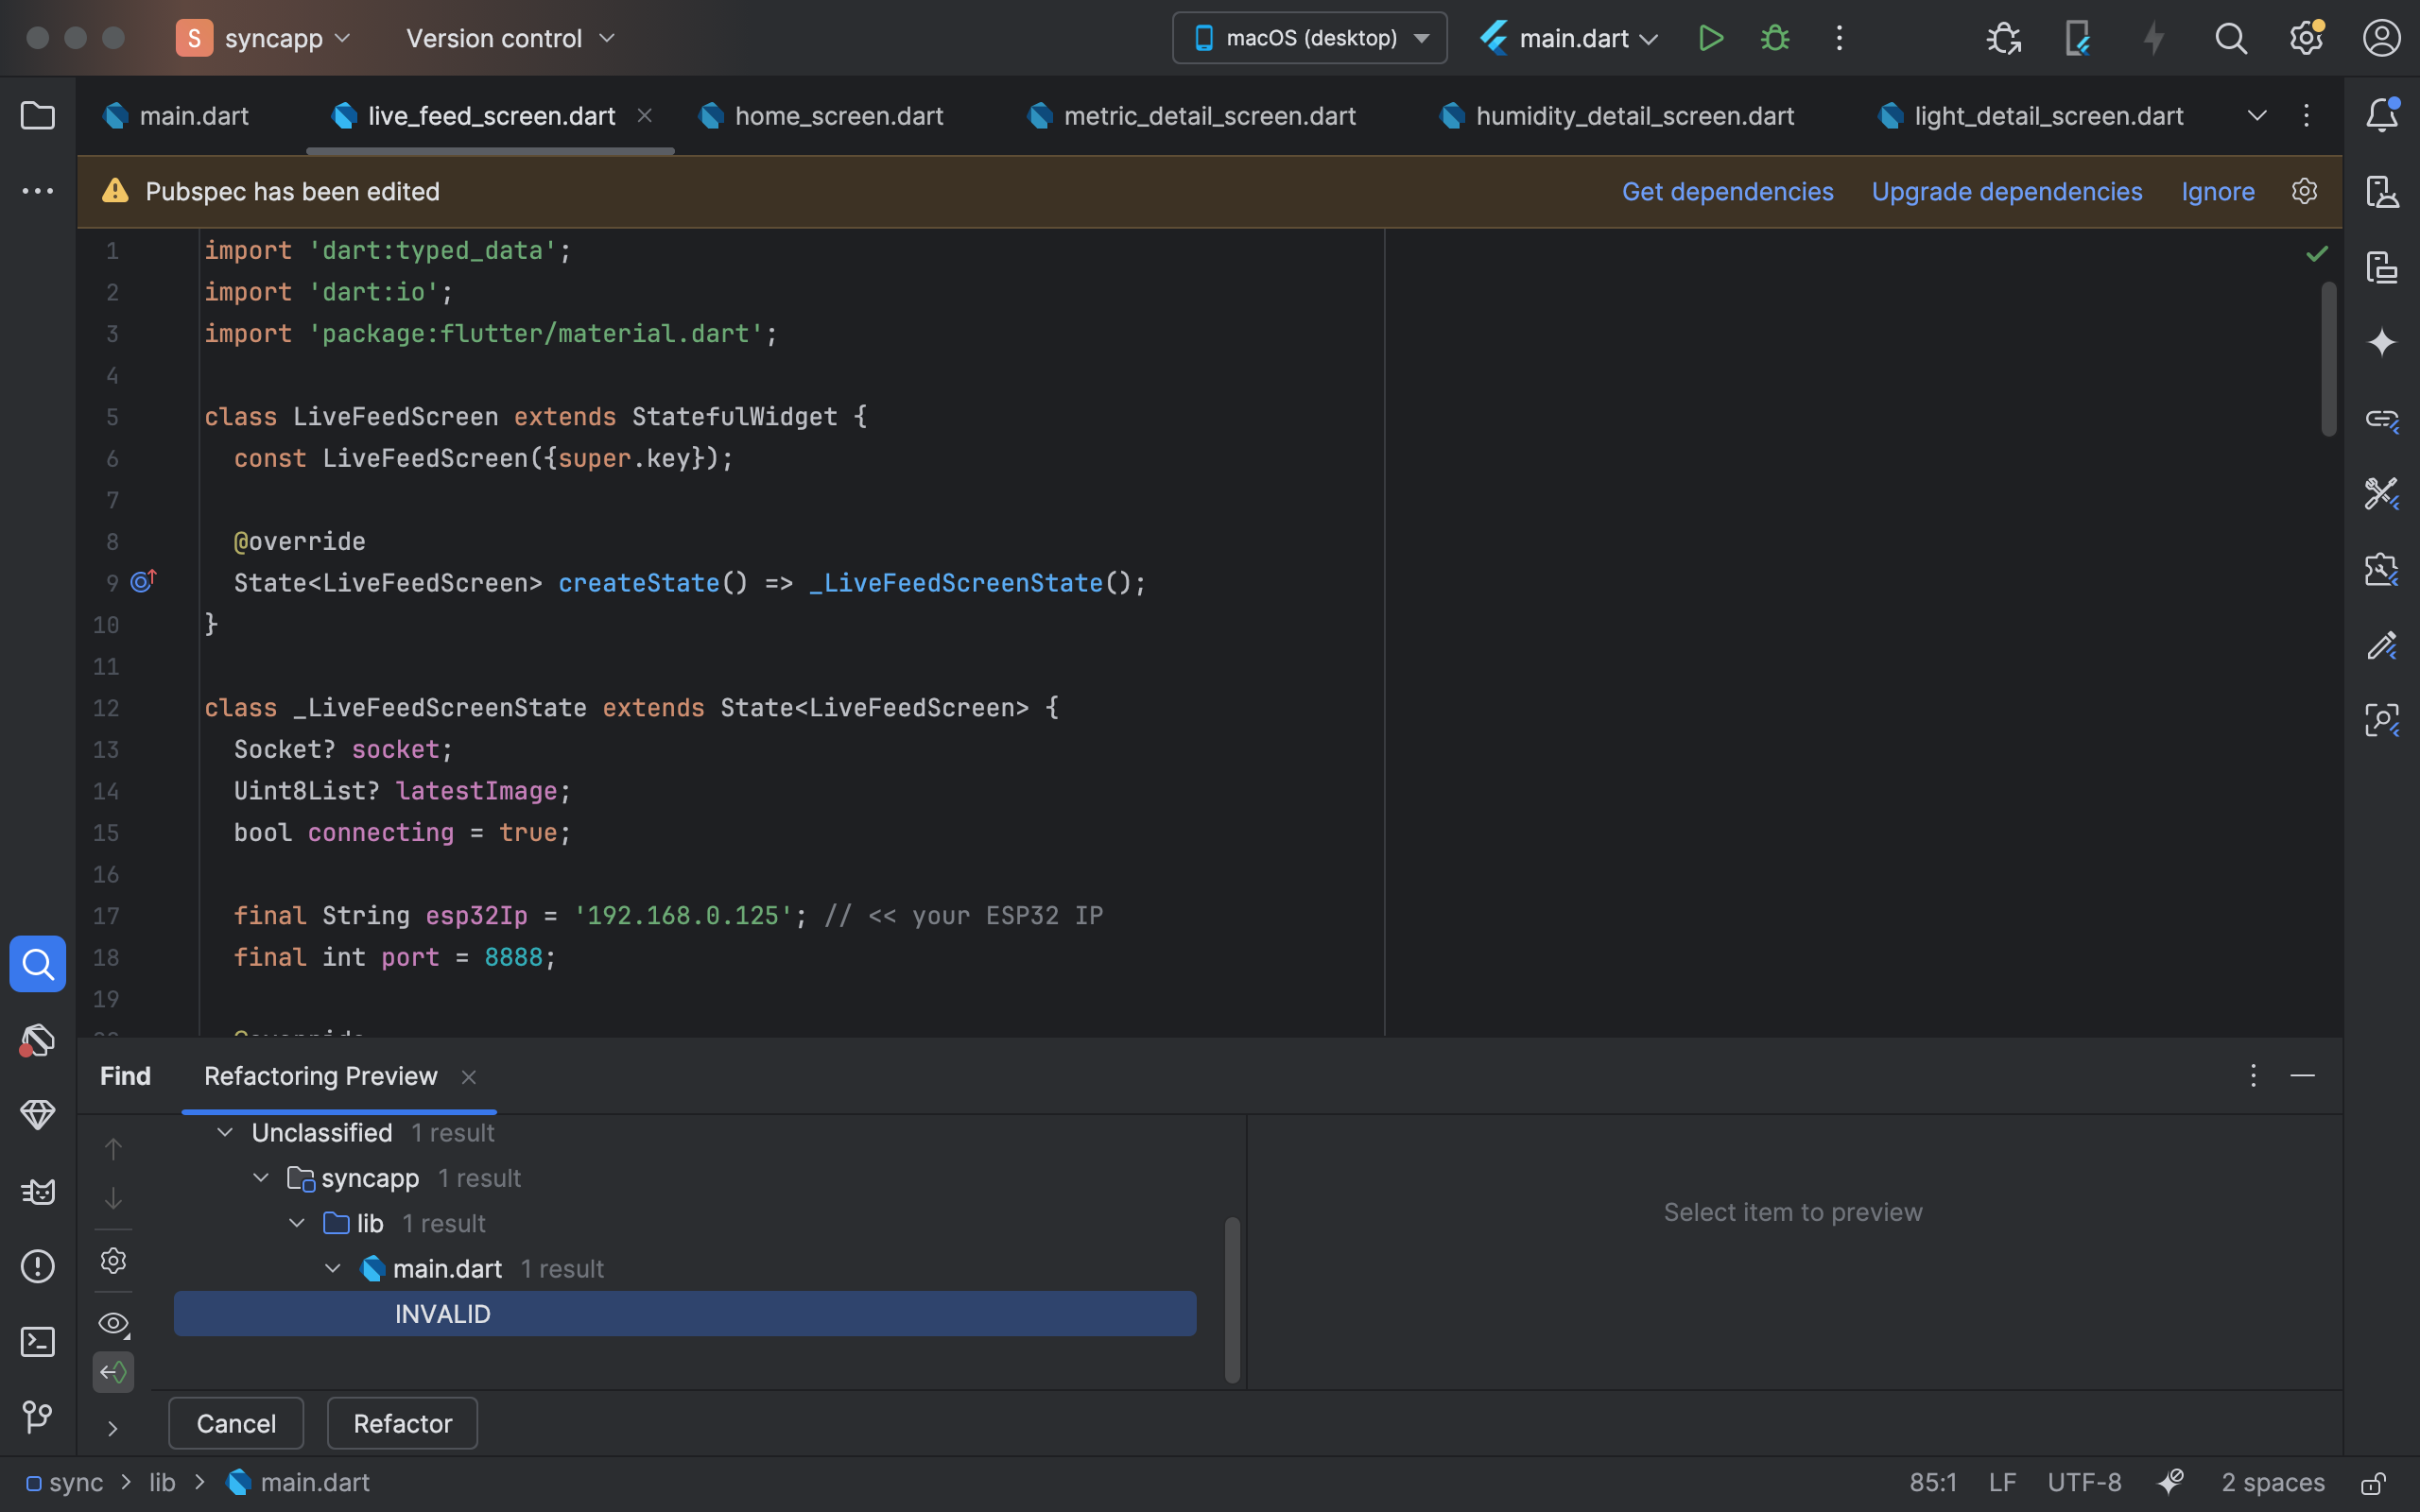
\includegraphics[width=0.8\textwidth]{ss.png}
\caption{Screenshot of Flutter TCP client code for ESP32-CAM live feed}
\end{figure}



\section{Technical Challenges and Solutions}

During development, dependency version conflicts in Flutter packages were resolved to maintain compatibility. Handling the real-time video stream efficiently required restructuring asynchronous data processing to prevent UI freezes. Additionally, the app’s codebase was organized modularly to allow straightforward integration of future features without disrupting existing functionality.

\section{Next Steps}

The immediate next steps include completing the live feed screen with fully stable connectivity, integrating the live feed into the Home Screen dashboard, testing end-to-end communication between the ESP32 sensors, actuators, and the mobile app, and implementing persistent data logging for both metrics and video stream to support future analytics and reporting.

\section{Conclusion}

This week’s work demonstrates significant progress in building a fully functional Seed Incubation Environmental Control App. The combination of detailed report generation, responsive Flutter screens, and preliminary live video feed integration sets a strong foundation for completing the app’s development in the coming weeks.

\end{document}
